\documentclass[journal]{IEEEtran}
\usepackage[pdftex]{graphicx}
\graphicspath{{../pdf/}{../jpeg/}}
\DeclareGraphicsExtensions{.pdf,.jpeg,.png}
\usepackage[cmex10]{amsmath}
\usepackage{array}
\usepackage{mdwmath}
\usepackage{mdwtab}
\usepackage{eqparbox}
\usepackage{url}
\usepackage{lipsum}
\usepackage{booktabs}
\usepackage{rotating}
\usepackage{graphicx}
\usepackage{multicol}
\usepackage{multirow}
\usepackage{listings} % code blocks
\usepackage{tabularx}
\usepackage{float}

\lstset{
  basicstyle={\small\ttfamily},
  breaklines=true,
  breakatwhitespace=true,
  tabsize=2
}

\renewcommand{\arraystretch}{1.25}

%=== TITLE & AUTHORS ====================================================================
\begin{document}
\title{An analysis of housing in California}
\author{
	Alisha Kartik,
	Ibrahim Khalid,
	Rahul Majmudar%
}
% The paper headers
\markboth{Housing in California}{Housing in California}


\maketitle



\begin{abstract}

	In recent years, the housing crisis in California has become a major problem
	for residents to contend with. In this project we explore the different
	facets that affect this issue from a housing affordability point of view as
	well as a demographic point of view. Then we will explore the future of
	housing by using time series analysis. From our analysis, we found that the
	housing crisis in California is only getting worse with time.

\end{abstract}

\begin{IEEEkeywords}
	Housing, California, Demographics, Analysis, Data Visualization, Time series analysis
\end{IEEEkeywords}

\IEEEpeerreviewmaketitle



% === I. INTRODUCTION =============================================================
% =================================================================================
\section{Introduction}

The housing affordability crisis is something that is affecting the day to day
lives of many Californians in a major way. There are many factors that play
into this, such as politics, land zoning, building regulations, market prices,
and population buying power. For our analysis, we will focus primarily on two
of these factors. The first is that the housing market in and of itself is
something that is running rampant, especially in cities in and around the San
Francisco Bay Area and the Los Angeles Metropolitan Area. The second factor
that we will be exploring is the disparity between housing affordability and
the buying power of the population. To get a better understanding of the
population, we choose to explore different segments of the population
demographics.

For exploration of the housing market, we turn to Zillow for the data. Zillow
is a well recognized organization that deals with housing in the United States.
It is primarily used by homeowners, buyers, and renters to list and purchase
housing. Due to this, Zillow has amassed a sizable amount of data regarding the
housing market. Zillow allows public access to this data in the form of
downloadable plain text files. There are a number of variables available on
Zillow, of them we use the Zillow Home Value Index (ZHVI), Zillow Market Heat
Index, and the Zillow New Homeowner Income Needed. We will explore the meaning
of each of these in the following section.

For understanding the demographics related to our problem statement, we first
needed to find a good variable to compare against. As we are exploring housing
affordability, we figure that personal income is a major contributing factor.
Our conjecture for selecting this variable is that the higher the income, the
more likely it is that the person will be able to afford a home. The dataset we
gathered comes from the United States Census dataset. By using these variables,
we will be able to get a holistic look at the problem we are trying to solve.

\section{Data Process}
The datasets used in this project include the following:
\begin{enumerate}

	\item Zillow Home Value Index (ZHVI): Monthly estimates of home values for
	      cities across  the United states.

	\item Zillow Affordability Index: Estimated income required to purchase a
	      house in the United states.

	\item Zillow Market Heat Index: Numerical metric to capture balance between
	      housing supply and demand.

	\item Demographic \& Personal Income Data: Population segmentation based on
	      age, gender, education level, race, income range, and population counts.

\end{enumerate}

The data preprocessing was done using pandas in python. All the datasets were
filtered for California city. The zillow dataset followed a format where the
first few columns were related to identification, such as State, City, and ID.
All columns after that related to a point in time and each cell represented the
value of that variable for that identifiable location at that point in time.
The ZHVI dataset contained monthly values from February 1996 to January 2025,
while the affordability dataset contained monthly values from January 2012 to
January 2025, and the market heat dataset contained monthly values from January
2018 to January 2025. By reading these three datasets into pandas, we were able
to perform the \lstinline{df.melt} command to go to a more traditional layout
with a date column and a value column. Using this format it was trivial to
combine the datasets on matching localities and dates. Due to the short range
of values for market heat, we combined it in a separate file, see Figure
\ref{fig:zillow-data}. For all the Zillow datasets, we limited the localities
to cities within California.

\begin{figure}[!htb]
	\centering
	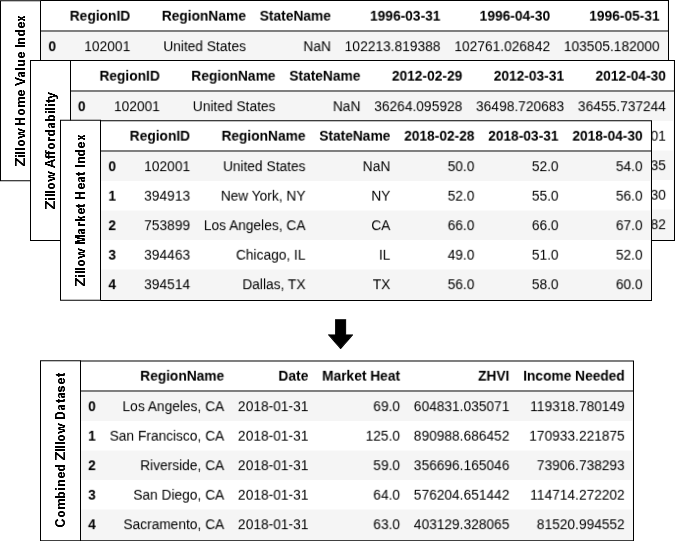
\includegraphics[width=\linewidth]{dataset-conversion.drawio.png}
	\caption{Filtering and combining the zillow data}
	\label{fig:zillow-data}
\end{figure}

The demographic data was downloaded separately per year for all years of
interest. The demographic data simply required us to concatenate the files
after adding a year column and cleaning up some of the data formats. The main
feature of this dataset is to find the number of people that fit under certain
descriptors. These descriptors are Year, Age, Gender, Education, Race, and
Personal Income. Due to Covid-19 related issues, the census data is not
available for the year 2020. Instead, we used simple interpolation of the
values from 2019 and 2021 to find them. See Figure \ref{fig:demo-data} for the
data format and Table \ref{tab:demo-cols} for the unique values present in the
dataset.

\begin{figure}[!htb]
	\centering
	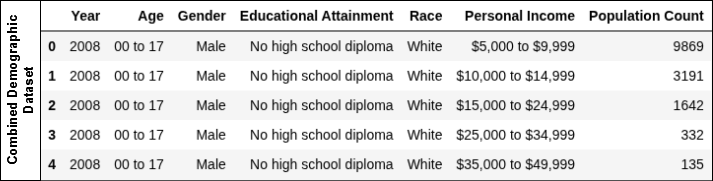
\includegraphics[width=\linewidth]{demographics.drawio.png}
	\caption{Combining the demographic dataset}
	\label{fig:demo-data}
\end{figure}

\begin{table*}[!htb]
	\caption{Values for each column in demographics dataset}
	\label{tab:demo-cols}
	\begin{tabularx}{\textwidth}{m{0.15\textwidth} X} % Adjust proportions as needed
		\toprule
		Column                 & Values                                                                                                                                                         \\
		\midrule
		Age                    & 00 to 17, 18 to 64, 65 to 80+                                                                                                                                  \\
		Gender                 & Male, Female                                                                                                                                                   \\
		Educational Attainment & No high school diploma, High school or equivalent, Some college, less than 4-yr degree, Bachelor's degree or higher                                            \\
		Race                   & White, African American, Asian, Hispanic, Other                                                                                                                \\
		Personal Income        & No Income, \$5,000 to \$9,999, \$10,000 to \$14,999, \$15,000 to \$24,999, \$25,000 to \$34,999, \$35,000 to \$49,999, \$50,000 to \$74,999, \$75,000 and over \\
		\bottomrule
	\end{tabularx}
\end{table*}

By analyzing the count of population demographics over the years and relating
this with the zillow datasets, we can find an understanding to our problem
statement.

\section{Data Exploration}
\subsection{Exploring demographic data}

We started our exploration with some simple analysis of population breakdown in
the demographic dataset. For a start, we want to see the breakdown of personal
income against different groups.

\begin{figure}[!htb]
	\centering
	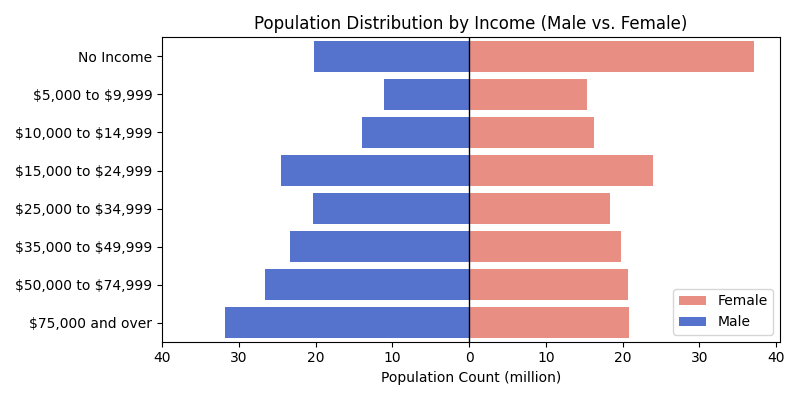
\includegraphics[width=\linewidth]{gender-income.png}
	\caption{Distribution of Gender at different income levels}
	\label{fig:gender-income}
\end{figure}

First, we looked at the difference between the genders when it comes to income
and we found that there were more men in higher income brackets as compared to
women, see Figure \ref{fig:gender-income}. This can be attributed to
traditional gender norms still being the prevalent default among couples. After
this, we looked at how different education levels stack up and we find that the
more a person is educated, the higher they will likely earn, see Figure
\ref{fig:edu-income}. Finally, we look at how different races in California
stack up in terms of income and found that white people earn more while African
American and Hispanics earn far less, see Figure \ref{fig:race-income}.
Interestingly, we find that Asians have a high presence in both lower and
higher income brackets.

\begin{figure}[!htb]
	\centering
	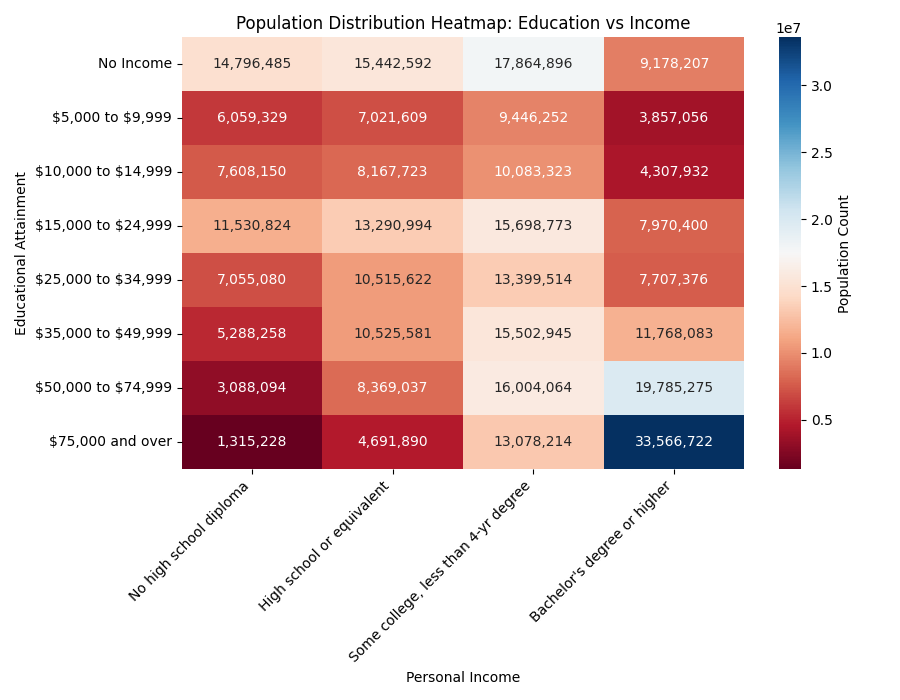
\includegraphics[width=1\linewidth]{edu-income.png}
	\caption{Distribution of Education levels at different income levels}
	\label{fig:edu-income}
\end{figure}

\begin{figure}[!htb]
	\centering
	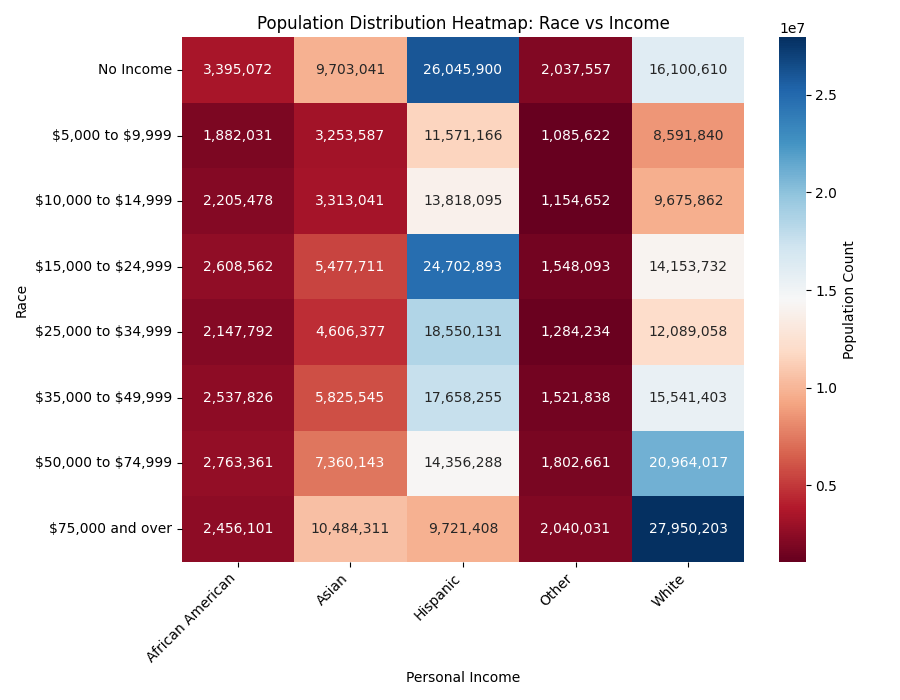
\includegraphics[width=1\linewidth]{race-income.png}
	\caption{Distribution of race group populations at different income levels}
	\label{fig:race-income}
\end{figure}


Next we looked at some variables over time, see Figure \ref{fig:ier-time}.
Firstly, we looked at the income distribution over time and found that
steadily, the number of people in California with an income of 75,000 or more
has gone up. We guess that this might be since people in lower income brackets
have been priced out of the market and have been forced to move somewhere else.
For education, the share of the low educated population has decreased over time
whereas the number of people with a bachelor's degree has gone up. This may be
due to the same reasoning as the income over time. Finally, we look at the
number of each racial group in California and see that besides whites and
Hispanics, the demographic breakdown remains the same. Over time, however, we
see there are a lot more Hispanics in California. This may be due to California
being more tolerant of people with diverse backgrounds and California’s
proximity to Mexico.

\begin{figure*}
	\centering
	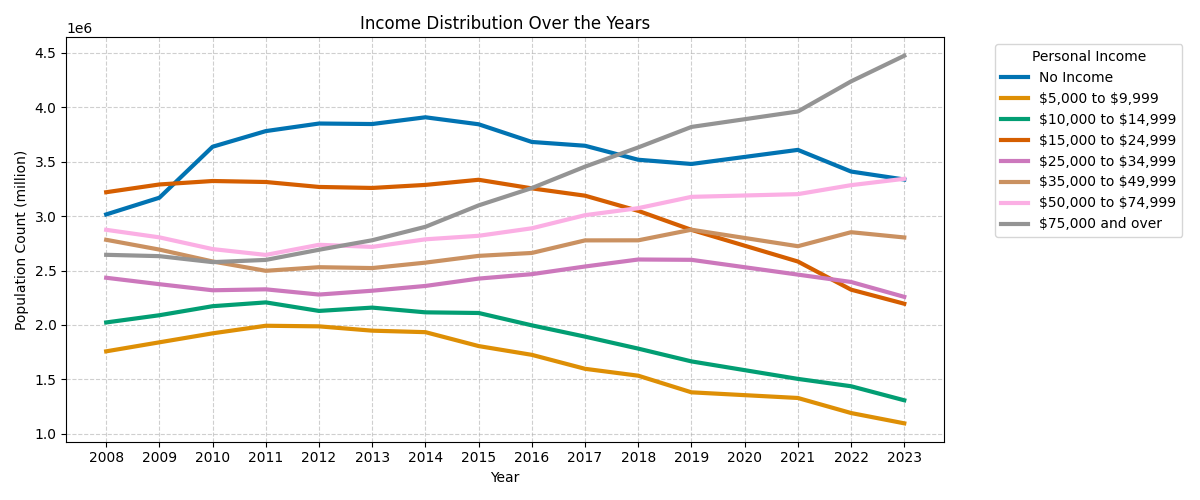
\includegraphics[width=1\linewidth]{income-time.png}
	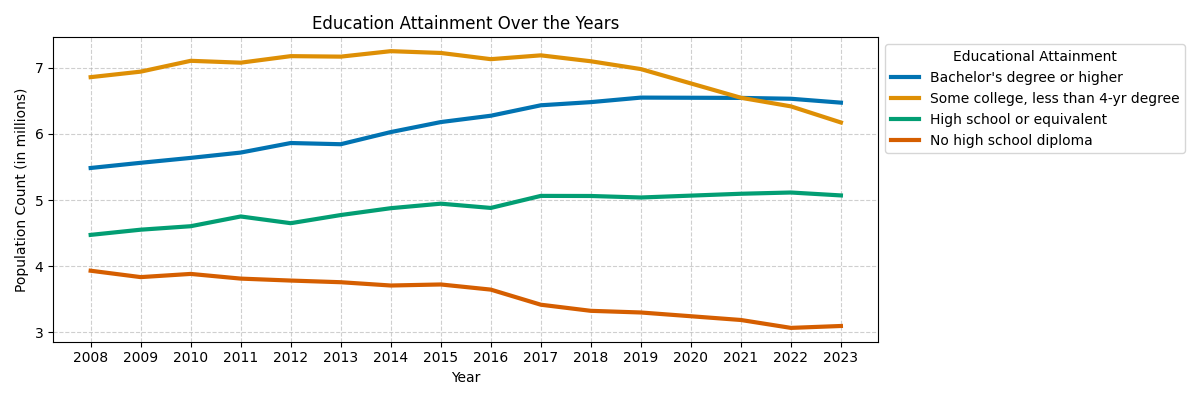
\includegraphics[width=1\linewidth]{edu-time.png}
	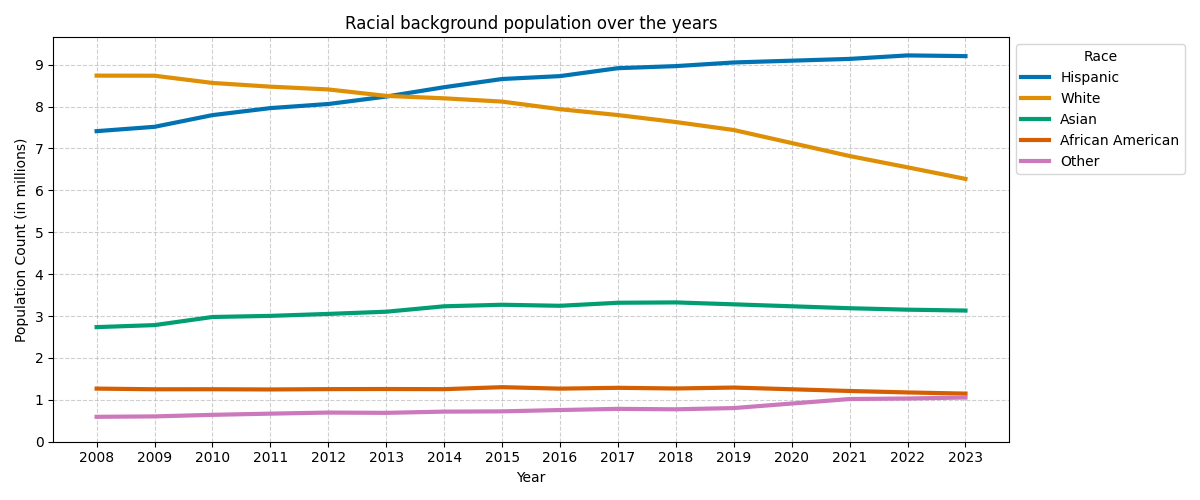
\includegraphics[width=1\linewidth]{race-time.png}
	\caption{Income, Education, and race over time}
	\label{fig:ier-time}
\end{figure*}

\subsection{Exploring housing data}

The Zillow datasets are one of the more important datasets we need to look at
to understand the problem at hand. We can start by looking at a list of all the
cities ranked by their home value index and its income needed, see Figures
\ref{fig:zhvi} and \ref{fig:income-needed}.

\begin{figure}
	\centering
	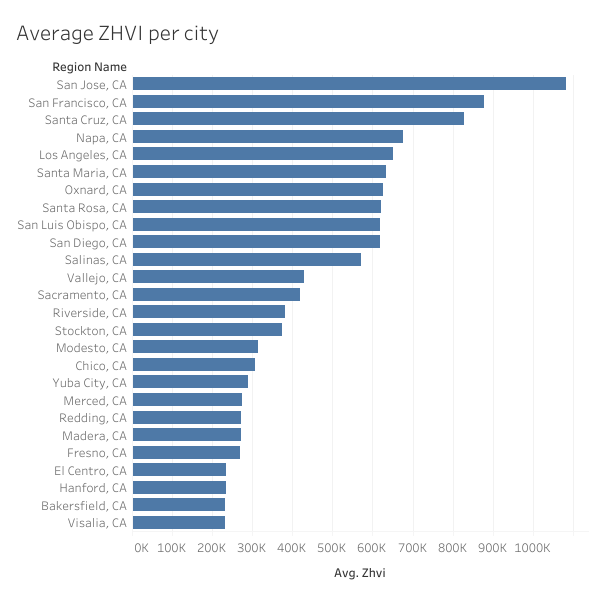
\includegraphics[width=\linewidth]{zhvi.png}
	\caption{Average Zillow home value index, ranked}
	\label{fig:zhvi}
\end{figure}

\begin{figure}
	\centering
	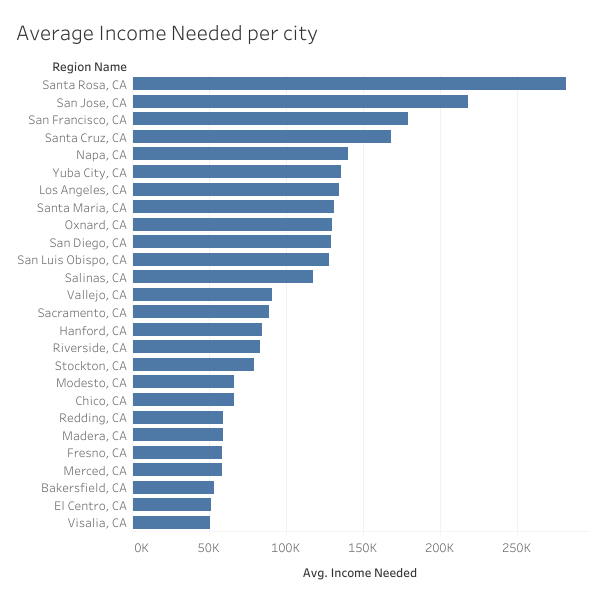
\includegraphics[width=\linewidth]{income-needed.png}
	\caption{Average income needed to buy a home, ranked}
	\label{fig:income-needed}
\end{figure}

We can see that the most expensive cities are San Jose, San Francisco, Santa
Rosa, and Santa Cruz, among others. Let’s have a closer look at how all these
cities are doing over time in terms of their ZHVI, see Figure \ref{fig:zhvi-year}.

\begin{figure}[!htb]
	\centering
	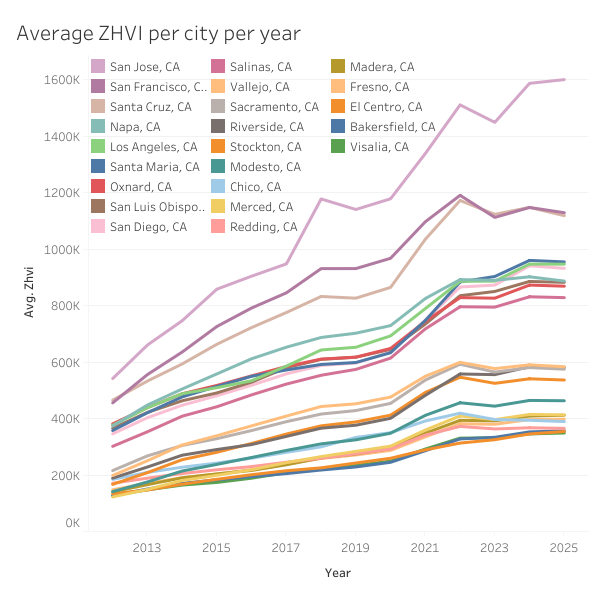
\includegraphics[width=1\linewidth]{zhvi-year.png}
	\caption{Average ZHVI per city per year}
	\label{fig:zhvi-year}
\end{figure}

Once again, we see that bay area cities are ranked the highest with San Jose
growing far faster than any other city in our dataset. For the rest of this
analysis, we will look at the following 5 cities, San Jose, San Francisco,
Santa Cruz, Napa, and Los Angeles. Comparing these cities with the state
average, we get the following graph. We also add the state average to the chart
to see how they all stack up. See Figure \ref{fig:zhvi-year-top}.

\begin{figure}
	\centering
	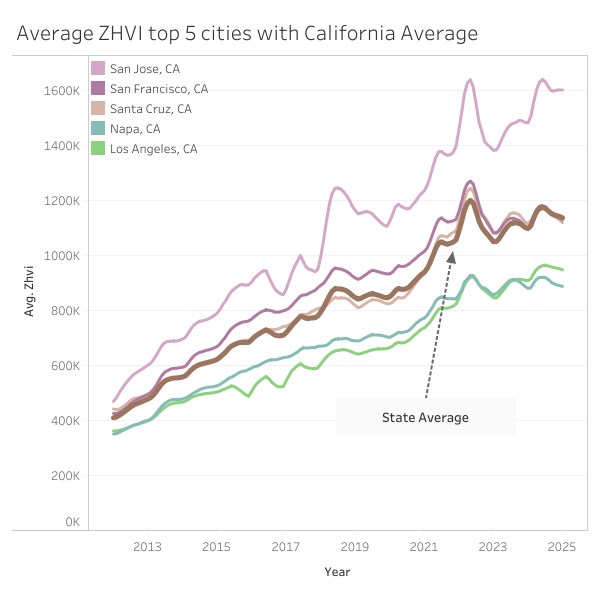
\includegraphics[width=1\linewidth]{zhvi-year-top5.png}
	\caption{Average ZHVI per city per year for top 5 cities along with the state average}
	\label{fig:zhvi-year-top}
\end{figure}

The graph in Figure \ref{fig:zhvi-income} shows the ratio between income needed
to buy a home and the average home value index for these 5 selected cities. A
value of 1 means that the income needed matches the value of a home. A value
more than 1 shows that you need more relative income than the value of the home
in order to buy it.

\begin{figure}
	\centering
	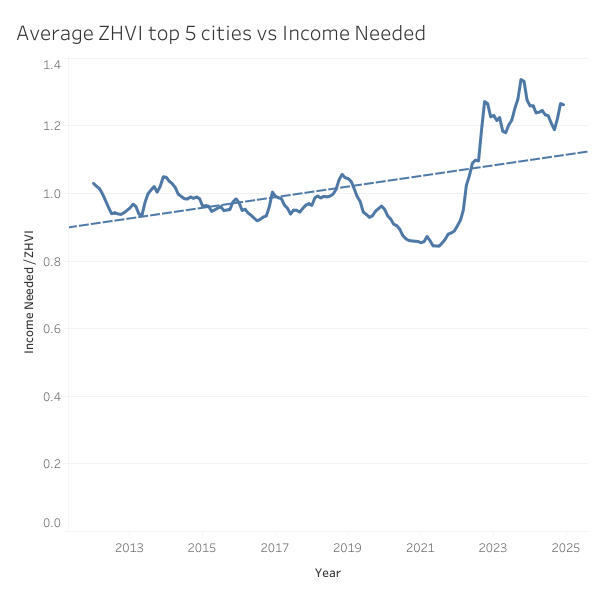
\includegraphics[width=1\linewidth]{zhvi-income.png}
	\caption{Ratio of income needed to buy a home and the average home value}
	\label{fig:zhvi-income}
\end{figure}

\section{Proposed Machine Learning Method}

The machine learning method we decided to use is ARIMA, or AutoRegressive
Integrated Moving Average. A quick summary of ARIMA: it's a very well-known
time series analysis tool, mainly used in the realm of economics (which fits
our project perfectly). The breakdown of ARIMA is as follows: AR or
Autoregressive uses the relationship between an observation and a number of
previous observations. I or Integrated, applies differencing to make
non-stationary data stationary by removing trends or seasonal effects. And
finally, MA, or moving average, takes the dependency between the observations
and errors from the previous predictions.

The model has three main configuration variables, p,d,q, which are associated
with each of the three components of ARIMA and can be used to fine-tune the
model based on the data it's used on. This method is well-suited for our
housing affordability analysis because it can pick up on short-term changes as
well as long-term trends. It is a staple ML method and has proven to be very
useful for gaining insights into our data.

\section{Results and Findings}

\subsection{Findings from the datasets}

Analyzing the Zillow and demographic datasets together indicates a strong
ongoing housing crisis. While some demographic groups are better situated to
handle the future market, the gap is widening between income and affordability.

\subsection{Machine Learning Results}

For our ML analysis, we systematically tested different ARIMA configurations
(p,d,q), from (0,0,0) to (2,2,2) to identify the optimal parameters for each
demographic in our demographics dataset, and for each region in our Zillow
dataset. The AIC or Akaike Information Criterion was measured with each
configuration to see which parameter set fit the model the best. Lower AIC
values indicate better model fit as well. The MAPE was used to gauge model
accuracy, and an accuracy of  98-99.7\% was seen across each demographic group
and Zillow predictions.

Now each of the forecasts for the Zillow dataset showed the average home value
climbing up in the near future, and the income needed increasing as well. For
example, San Jose is projected to reach an average home value of \$1.9M by
2028. Los Angeles is also predicted to reach an average of \$1M in home value
by 2028, however, there is a clear divergence as the predictions seem to favor
San Jose house values to skyrocket compared to any other region. The other top
regions’ ZHVI do seem to level off, however, the income needed is projected to
increase for all top regions. See Figure \ref{fig:arima-zillow}.

For the demographics forecast, we see the Hispanic population overtaking the
White population by 2028. The high-income and low-income groups are expanding,
while the middle-income group shrinks. For age, the seniors (65+) show
consistent growth whereas the youth in California remains the same. And for the
total population forecast, after a recent decline, it predicts the population
to stabilize, which makes sense as the exodus from California during the
pandemic is now over, and the population decline is now in a state of
correction. See Figure \ref{fig:arima-demo}.

\begin{figure*}[!htb]
	\centering
	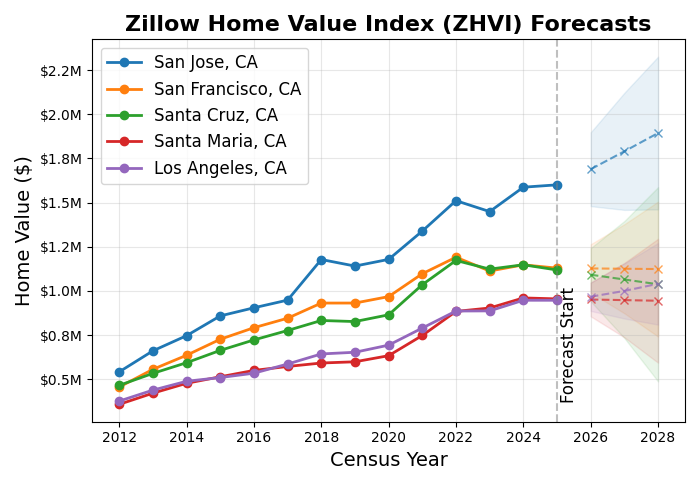
\includegraphics[width=0.45\linewidth]{zhvi_forecasts.png}
	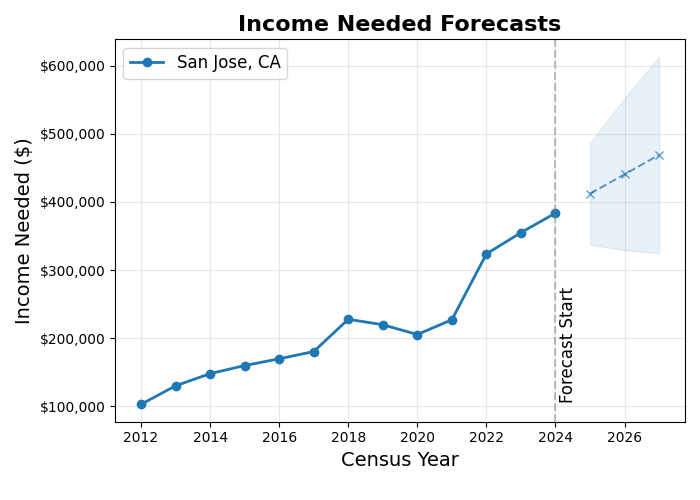
\includegraphics[width=0.45\linewidth]{income_needed_forecasts.png}
	\caption{ARIMA forecasts for ZHVI and Income Needed in California until 2028}
	\label{fig:arima-zillow}
\end{figure*}

\begin{figure*}[!htb]
	\centering
	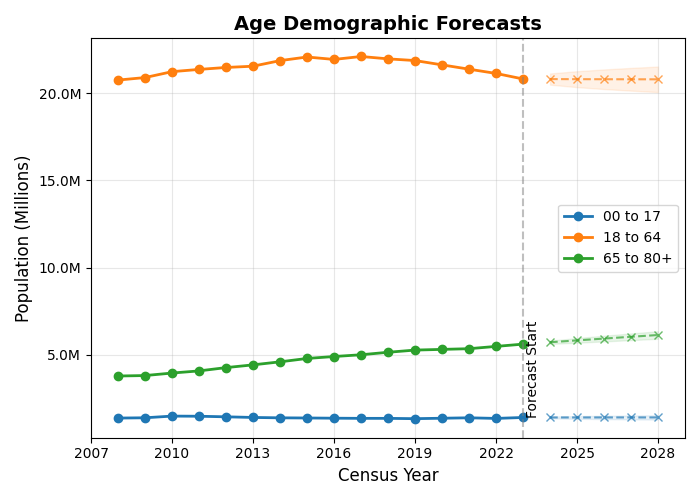
\includegraphics[width=0.45\linewidth]{age_demographics_forecast.png}
	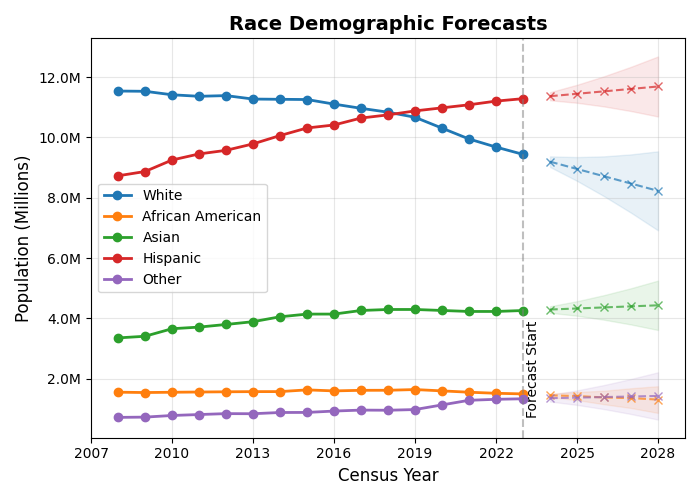
\includegraphics[width=0.45\linewidth]{race_demographics_forecast.png}
	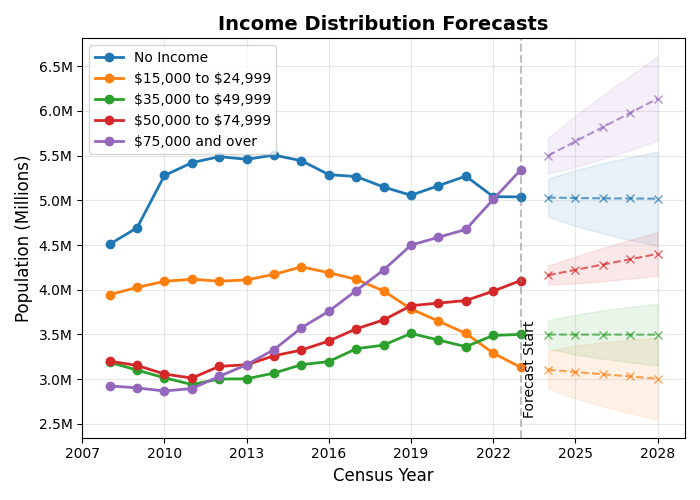
\includegraphics[width=0.45\linewidth]{income_distribution_forecast.png}
	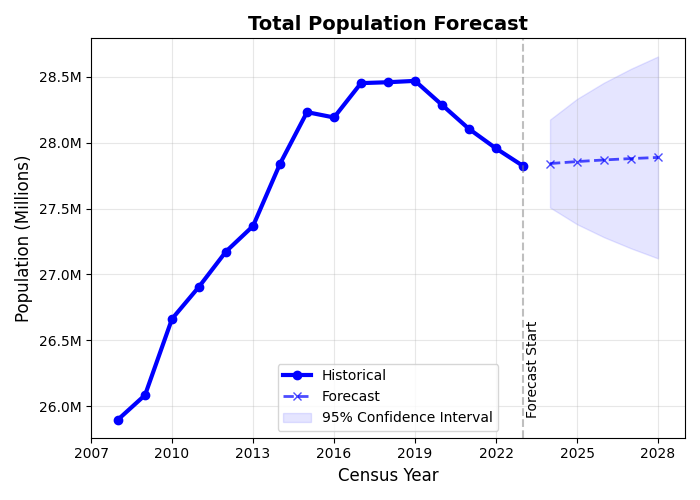
\includegraphics[width=0.45\linewidth]{total_population_forecast.png}
	\caption{ARIMA forecasts for all demographic groups in California until 2028}
	\label{fig:arima-demo}
\end{figure*}


\section{Conclusion}

To summarize our findings, the housing affordability in California is getting
worse. It was already in a poor state, however, home values are showing trends
of increasing while the income needed to afford these houses isn’t relenting at
all. The ARIMA forecasting analysis highlights the growing wage gap between the
rich and the poor, along with a shrinking middle class, thus allowing a smaller
population to become homeowners in California.

Our advice for the average Californian: save your money! Do not buy a house in
California; it's best to rent cheaply in the short term and, when possible,
move to a more affordable location in the future.


\end{document}
